\chapter{The menus}\label{ch:menus}

This chapter goes through the menu bar. The table of every command with its key and its short description is in
appendix~\ref{app:reference} (it is written by the program, so it is always up to date); here each menu is shown and the commands
that need an explanation are explained.

\section{File}

\begin{minipage}[t]{0.38\textwidth}\vspace{0pt}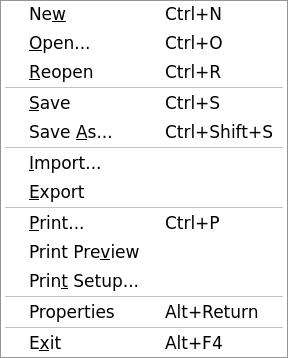
\includegraphics[width=\textwidth]{images/menu-File.png}\end{minipage}\hfill
\begin{minipage}[t]{0.58\textwidth}\vspace{0pt}
\begin{itemize}[leftmargin=1em]
  \item \menu{New}, \menu{Open\ldots}, \menu{Reopen} (loads the song from the last saved version), \menu{Save}, \menu{Save As\ldots}:
        the song is an \texttt{.rmt} file; \texttt{.txt} and \texttt{.rmw} are chosen in the file type of the dialog.
  \item \menu{Import\ldots}: ProTracker modules and TMC songs (chapter~\ref{ch:importexport}).
  \item \menu{Export}: the formats for the Atari (chapter~\ref{ch:importexport}).
  \item \menu{Print}, \menu{Print Preview}, \menu{Print Setup}: the screen of the song is printed on a landscape page, scaled to fill it.
  \item \menu{Properties} (\key{ALT+ENTER}): the properties of the song.
\end{itemize}
\end{minipage}

\section{Edit}

\begin{minipage}[t]{0.5\textwidth}\vspace{0pt}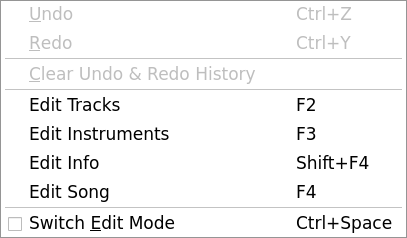
\includegraphics[width=\textwidth]{images/menu-Edit.png}\end{minipage}\hfill
\begin{minipage}[t]{0.46\textwidth}\vspace{0pt}
Undo and redo (the history can be cleared), the four parts of the screen (tracks, instruments, info, song), and the switch between
edit and prove mode.
\end{minipage}

\section{View}

\begin{minipage}[t]{0.36\textwidth}\vspace{0pt}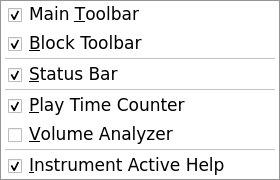
\includegraphics[width=\textwidth]{images/menu-View.png}\end{minipage}\hfill
\begin{minipage}[t]{0.6\textwidth}\vspace{0pt}
Shows or hides the toolbars and the status bar, the play time counter, the volume analyzer and the instrument active help. The
choices are kept in the configuration.
\end{minipage}

\section{Play}

\begin{minipage}[t]{0.5\textwidth}\vspace{0pt}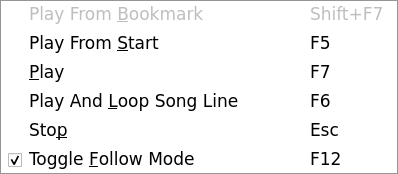
\includegraphics[width=\textwidth]{images/menu-Play.png}\end{minipage}\hfill
\begin{minipage}[t]{0.46\textwidth}\vspace{0pt}
Play from the bookmark, from the start, from the cursor, loop the song line, stop and follow mode (chapter~\ref{ch:playing}).
\end{minipage}

\section{Channels}

\begin{minipage}[t]{0.5\textwidth}\vspace{0pt}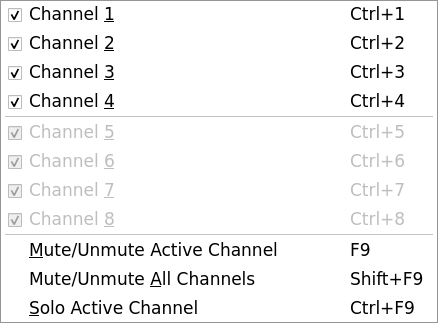
\includegraphics[width=\textwidth]{images/menu-Channels.png}\end{minipage}\hfill
\begin{minipage}[t]{0.46\textwidth}\vspace{0pt}
Switch on and off each of the channels 1 to 8, mute or unmute the active one or all of them, or play the active one alone.
\end{minipage}

\section{Song}

\begin{minipage}[t]{0.58\textwidth}\vspace{0pt}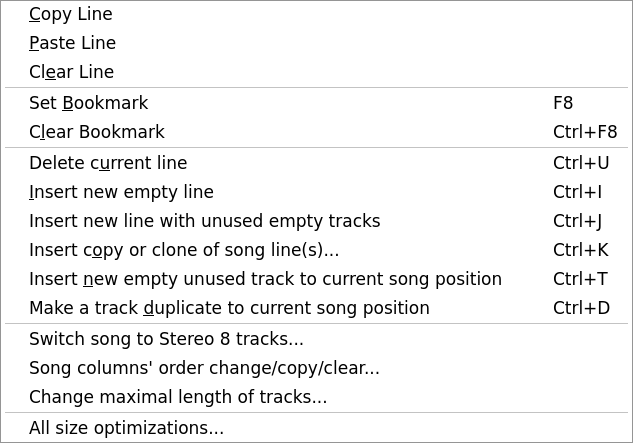
\includegraphics[width=\textwidth]{images/menu-Song.png}\end{minipage}\hfill
\begin{minipage}[t]{0.38\textwidth}\vspace{0pt}
Copy, paste and clear a song line; the bookmark; insert and delete lines; insert tracks; and the commands of chapter~\ref{ch:song}
that change the whole song.
\end{minipage}

\section{Instrument}

\begin{minipage}[t]{0.5\textwidth}\vspace{0pt}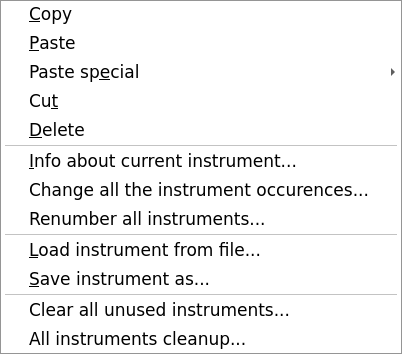
\includegraphics[width=\textwidth]{images/menu-Instrument.png}\end{minipage}\hfill
\begin{minipage}[t]{0.46\textwidth}\vspace{0pt}
Everything to do with an instrument: copy and paste (and paste special), information, change or renumber, clear the unused ones,
load and save (chapter~\ref{ch:instruments}).
\end{minipage}

\section{Track}

\begin{minipage}[t]{0.58\textwidth}\vspace{0pt}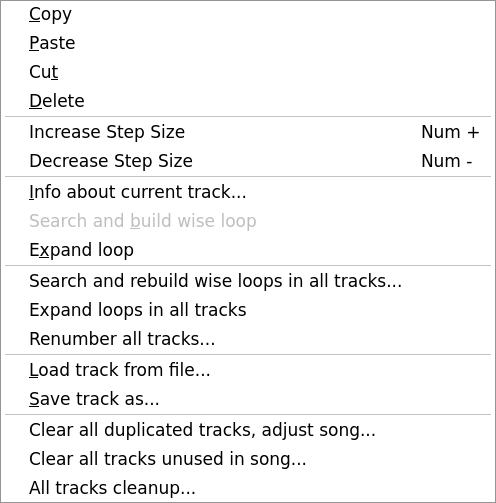
\includegraphics[width=\textwidth]{images/menu-Track.png}\end{minipage}\hfill
\begin{minipage}[t]{0.38\textwidth}\vspace{0pt}
Copy, paste, cut and delete a track; the step size; information about the current track; wise loops; renumbering; loading and saving a
track; and the clean-up of the tracks of the song.
\end{minipage}

\section{Block}

\begin{minipage}[t]{0.5\textwidth}\vspace{0pt}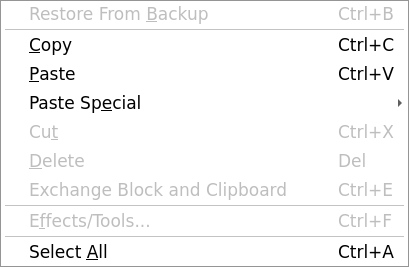
\includegraphics[width=\textwidth]{images/menu-Block.png}\end{minipage}\hfill
\begin{minipage}[t]{0.46\textwidth}\vspace{0pt}
The commands of the blocks (chapter~\ref{ch:tracks}): restore from the backup, copy, paste, paste special (merge, only the volumes, only the
speeds), cut, delete, exchange, effects and tools, select all.
\end{minipage}

\section{Pokey}

\begin{minipage}[t]{0.58\textwidth}\vspace{0pt}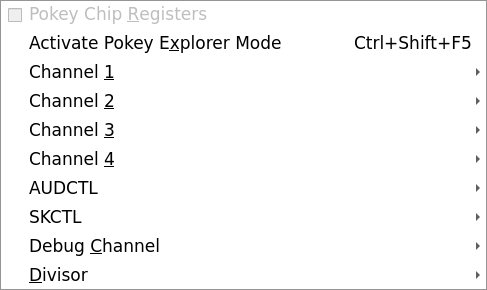
\includegraphics[width=\textwidth]{images/menu-Pokey.png}\end{minipage}\hfill
\begin{minipage}[t]{0.38\textwidth}\vspace{0pt}
The registers of the chip and the Pokey explorer mode, with a submenu for each channel (chapter~\ref{ch:explorer}).
\end{minipage}

\section{Tools}

\begin{minipage}[t]{0.35\textwidth}\vspace{0pt}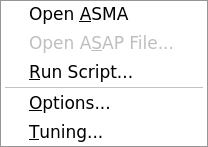
\includegraphics[width=\textwidth]{images/menu-Tools.png}\end{minipage}\hfill
\begin{minipage}[t]{0.61\textwidth}\vspace{0pt}
\menu{Open ASMA} opens the Atari SAP Music Archive in the browser; \menu{Run Script\ldots} runs a script
(chapter~\ref{ch:scripting}); \menu{Options\ldots} and \menu{Tuning\ldots} open the dialogs of chapter~\ref{ch:options}.
\end{minipage}

\section{Help}

\begin{minipage}[t]{0.32\textwidth}\vspace{0pt}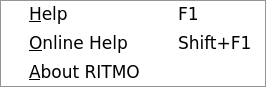
\includegraphics[width=\textwidth]{images/menu-Help.png}\end{minipage}\hfill
\begin{minipage}[t]{0.64\textwidth}\vspace{0pt}
The online help (a browser page with the documentation) and the \menu{About} window, with the credits.
\end{minipage}
